%----------------------------------------------------------------------------
%
% 
% 
%
%----------------------------------------------------------------------------
%----------------------------------------------------------------------------
%----------------------------------------------------------------------------

\ProvidesFile{proposal.tex}
\documentclass[cameraready]{acmsiggraph-awb}
\usepackage[scaled=.92]{helvet}
\usepackage{times}
\usepackage{algorithm}
\usepackage{algorithmic}

\usepackage[pdftex]{graphicx} \pdfcompresslevel=9

\usepackage{parskip}

\usepackage[labelfont=bf,textfont=it]{caption}

\usepackage{amsmath}
\usepackage{amssymb}
\usepackage{wasysym}
\usepackage{bm}
\usepackage{cite}

\usepackage{enumerate}

\usepackage{url}

% For backwards compatibility to old LaTeX type font selection.
% Uncomment if your document adheres to LaTeX2e recommendations.
\let\rm=\rmfamily    \let\sf=\sffamily    \let\tt=\ttfamily
\let\it=\itshape     \let\sl=\slshape     \let\sc=\scshape
\let\bf=\bfseries

% end of prologue
\usepackage[%
 breaklinks,
 letterpaper,
 bookmarks,
 bookmarksnumbered,
 colorlinks,
 linkcolor={black},
 citecolor={black},
 pdfpagemode={None},
]{hyperref}
\setlength\paperwidth{8.5in}  % Override any random settings...
\setlength\paperheight{11in}

\DeclareMathOperator*{\argmin}{\arg\!\min}


\newcommand{\etal}{et al.}
\newcommand{\hidecomment}[1]{}
\newcommand{\Mueller}{M\"{u}ller\ }
\newcommand{\Bez}{B\'{e}zier\ }
\newcommand{\BM}[1]{\B{#1}}
%\newcommand{\B}[1]{\mbox{\boldmath$#1$}}
%\newcommand{\B}[1]{\textbf{\textit{#1}}}
\newcommand{\B}[1]{\mathit{\mathbf{#1}}}
%\newcommand{\B}[1]{\boldsymbol{#1}}
\newcommand{\Per}{\%}
\newcommand{\Unit}[1]{{\mbox{$\,\mathrm{#1}$}}}
\newcommand{\Snit}[1]{{\mbox{\small$\mathrm{#1}$}}}
\newcommand{\Tr}[1]{\mathrm{Tr}\left(#1\right)}
\newcommand{\Hz}{\Unit{Hz}}
\newcommand{\MHz}{\Unit{MHz}}
\newcommand{\GHz}{\Unit{GHz}}
\newcommand{\Sec}{\Unit{sec}}
\newcommand{\SPF}{\Unit{sec/frame}}
\newcommand{\Min}{\Unit{min}}
\newcommand{\Max}{\Unit{max}}
\newcommand{\M}{\Unit{m}}
\newcommand{\Nab}{\B{\nabla}}
\newcommand{\TP}{^\mathsf{T}}

\newcommand{\Dist}{\mbox{dist}}

\newcommand{\figureTopBot}[1]{
  \begin{figure}[!tb]{\sloppy #1}\end{figure}
}

\newcommand{\figureTop}[1]{
  \begin{figure}[!t]{\sloppy #1}\end{figure}
}
 
\newcommand{\figureBot}[1]{
  \begin{figure}[!b]{\sloppy #1}\end{figure}
}

\newcommand{\figureWideTop}[1]{
  \begin{figure*}[!t]{\sloppy #1}\end{figure*}
}

\newcommand{\eqAlgn}{\!\!&\!\!}

\newcommand{\Eref}[1]{Equation~(\ref{#1})}
\newcommand{\Erefs}[2]{Equations~(\ref{#1}) and (\ref{#2})}
\newcommand{\eref}[1]{Equation~(\ref{#1})}
\newcommand{\erefs}[2]{Equations~(\ref{#1}) and (\ref{#2})}
\newcommand{\Sref}[1]{Section~\ref{#1}}
\newcommand{\sref}[1]{Section~\ref{#1}}
\newcommand{\fref}[1]{Figure~\ref{#1}}
\newcommand{\frefAND}[2]{Figures~\ref{#1} and~\ref{#2}}
\newcommand{\frefs}[2]{Figures~\ref{#1} and~\ref{#2}}
\newcommand{\frefss}[3]{Figures~\ref{#1}, \ref{#2}, and~\ref{#3}}
\newcommand{\Fref}[1]{Figure~\ref{#1}}
\newcommand{\Frefs}[2]{Figures~\ref{#1} and~\ref{#2}}
\newcommand{\Frefss}[3]{Figures~\ref{#1}, \ref{#2}, and~\ref{#3}}
\newcommand{\tref}[1]{Table~\ref{#1}}

\renewcommand{\labelenumi}{\arabic{enumi}.}
\renewcommand{\labelenumii}{\alph{enumii}.}
\renewcommand{\labelenumiii}{\roman{enumiii}.}

\newenvironment{algstep}{%
  \begin{enumerate}%
    \setlength{\itemsep}{0in}%
    \setlength{\partopsep}{0in}%
    \setlength{\topsep}{0in}%
}{\end{enumerate}}





\onlineid{papers\_0632}
\newcommand{\theTitle}{GPU Accelerated Point-Based Elastoplastic Solid Simulation}

\title{\theTitle}

\author{
	Ben Jones \and Kyle Hansen}

\newcommand{\theKeywords}{%
  viscoelastic materials, point-based animation, natural phenomena, physics-based animation.%
}


\begin{document}

\teaser{\begin{centering}
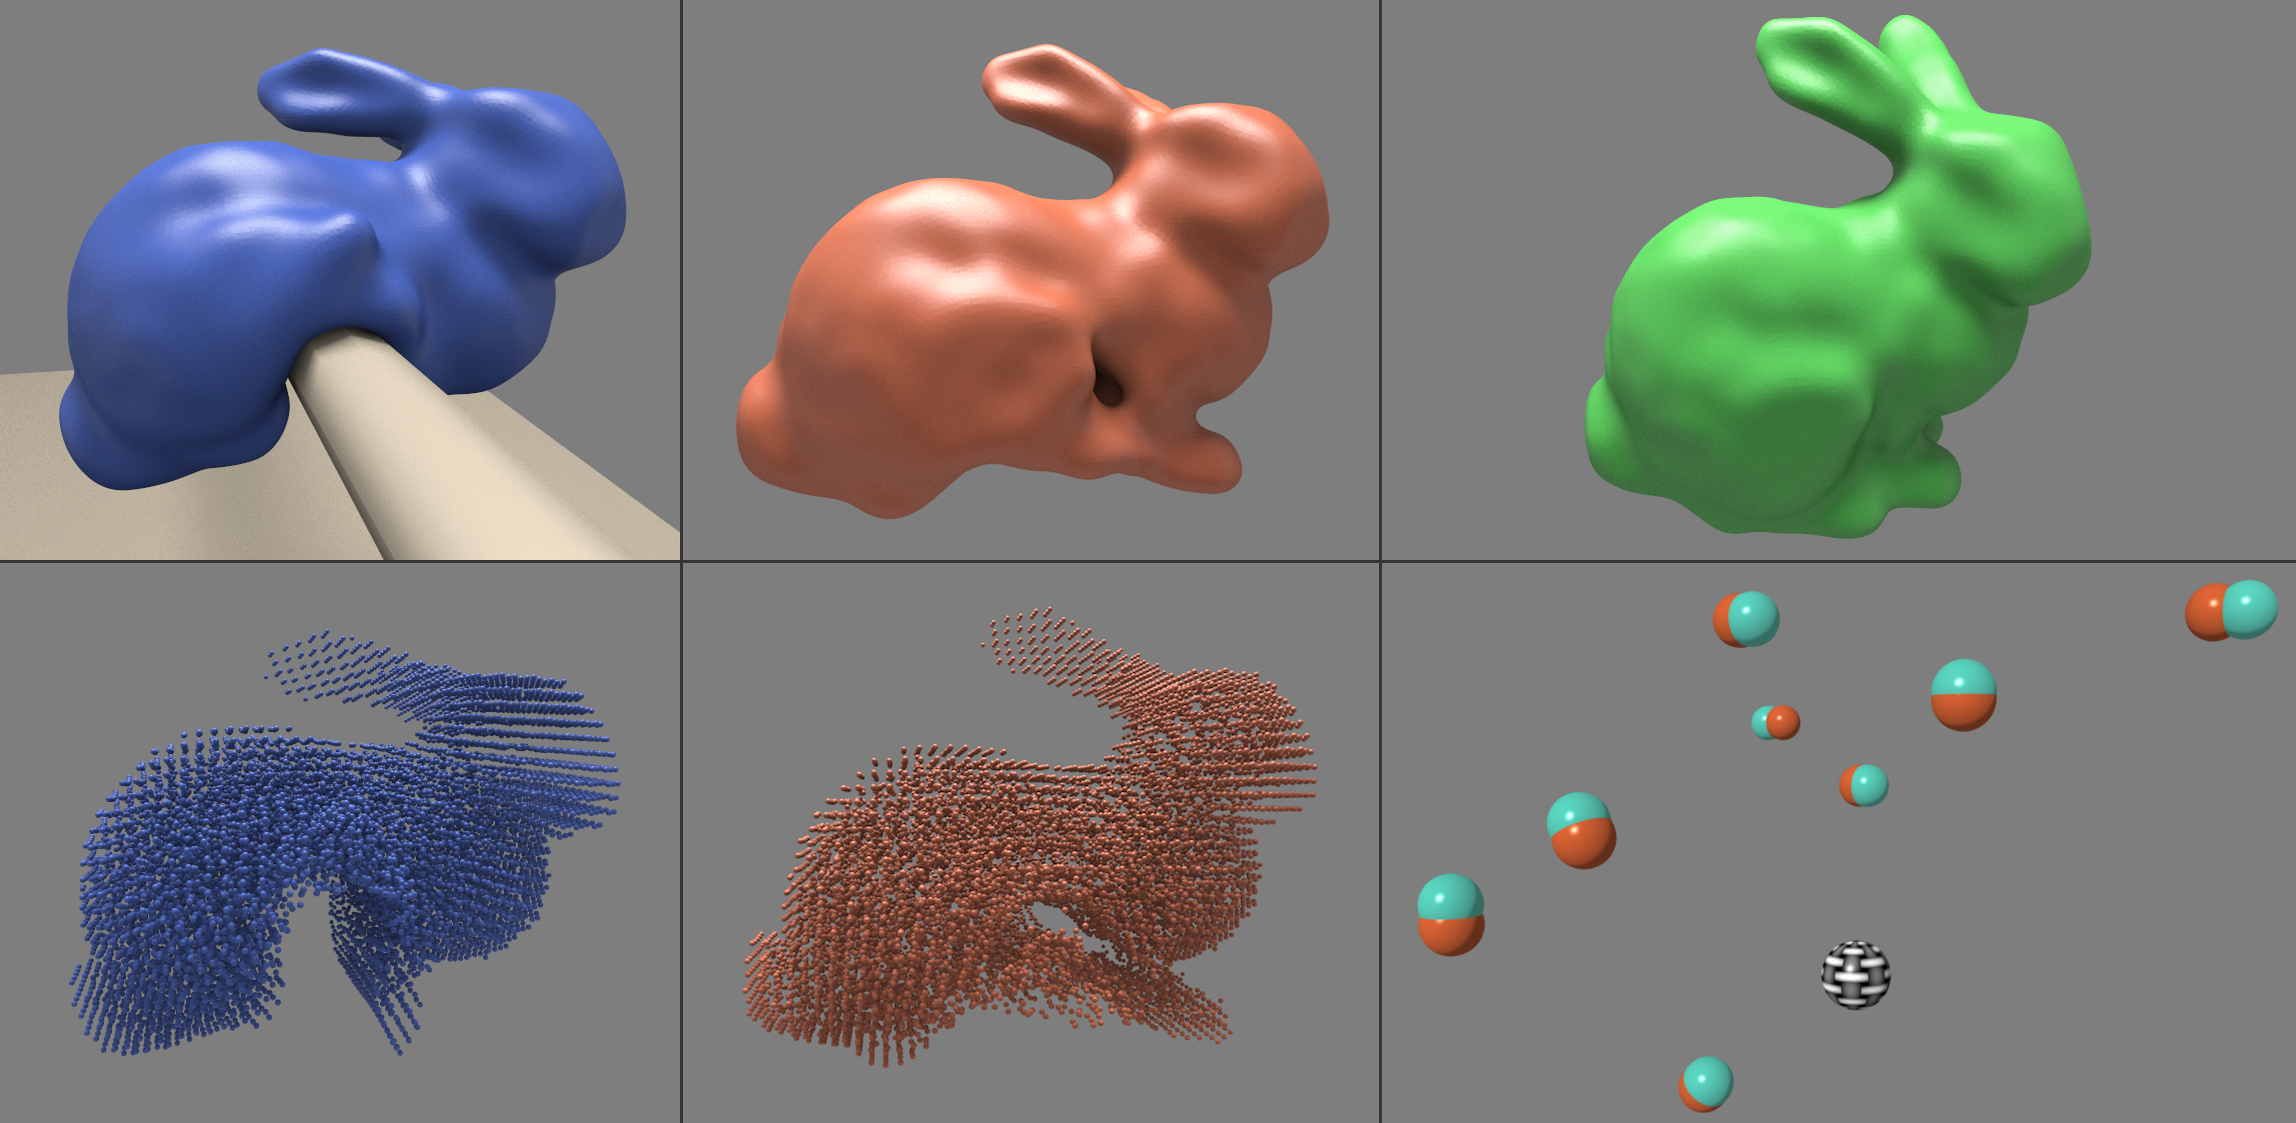
\includegraphics[width=6.1in]{Figures/teaser.png}
\caption{Sample frames from a sequential, point-based elastoplastic simulator, which is being accelerated with a GPU implementation for this project.}
\label{fig:teaser}
\end{centering}
}

\maketitle




\section{Team members}

\begin{itemize}

\item Ben Jones: Part of the team that implemented the sequential version of this algorithm, working with Adam Bargteil on graphics simulation research.
Will be focusing on the core algorithm parallelization.

\item Kyle Hansen: Computing Masters Student in the Graphics and Visualization Track.  
2+ years of real world programming experience as an electronics engineer.  
Hobby game programmer.  
Will be primarily concerned with the real time openGL rendering of simulation results and nearest neighbor calculations.

\end{itemize}

\section{Problem Description}

Simulating deformable solids is important for creating visual effects.  To generate compelling effects, we need to be able to handle materials across the entire spectrum from highly elastic, to totally plastic.  Using finite element methods with volumetric meshes (often tetrahedral) is a common approach, but large plastic deformation creates poorly conditioned tetrahedra.  To handle this, complicated volumetric remeshing is necessary to maintain stability and accuracy.  Recently, several point based methods have been proposed to avoid these expensive/complex operations.  However, these methods often support only one end of the spectrum, elastic or plastic materials, but not both  \cite{Mueller:2004:PBA}, \cite{Gerszewski:2009:APB}.  Recently, Jones et al. \cite{us} proposed a new point based technique that handles materials across the range between elastic and plastic.  The goal of our project is to improve performance of their method by performing as much computation as possible on the GPU.  

\section{Algorithm Description}

During elastoplastic simulation, deformation is computed by comparing the current deformed configuration of point samples with their reference configuration.  This deformation, along with material properties, is used compute elastic forces and plastic deformation of the reference configuration.  This is shown schematically in Figure \ref{fig:defGrad}.
\begin{figure}
\begin{centering}
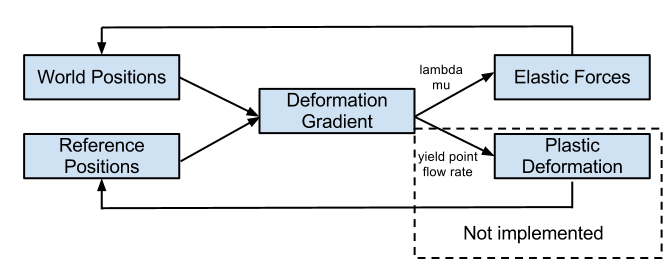
\includegraphics[width = 5in]{Figures/algSchematic.png}
\caption{The difference between world and reference configurations defines the deformation gradient, which, along with material parameters, defines elastic forces and plastic deformation.}
\label{fig:defGrad}
\end{centering}
\end{figure}


During the simulation, we maintain the objects world configuration, a set of nearest neighbors for each particle, and least squares fit of the global reference configuration.  At each simulation time step, we perform the following steps:
\begin{itemize}

\item compute deformation gradient, per particle
\begin{itemize}
\item factor gradient into elastic and plastic components
\item apply elastic and body (gravity) forces
\item apply plastic deformation to vectors to all neighbors of a particle*
\end{itemize}
\item integrate elastic forces
\begin{itemize}
\item perform explicit integration step of elastic and body forces
\item perform implicit damping force solve* 
\end{itemize}
\item compute new world reference configuration* 
\item compute per particle local error in global reference configuration* 
\item update particle neighborhoods 
\item resolve obstacle collisions
\item render current simulation frame (using openGL)**
\item write particle positions to file*
\end{itemize}

* Not yet included in the CUDA implementation.

** Unique to the CUDA implementation.

For more details please refer to \cite{us}.
It should be noted that the above steps outline the complete simulation algorithm, which has not all been implemented for this particular project.
For this project, we have only considered the elastic and body forces while also accelerating the K nearest neighbor (KNN) calculations and incorporating OpenGL to render the results as they are calculated.
The primary goal for this project is to illustrate the potential acceleration that could be acheived by incorporating CUDA parallelization into the simulation.


\section{Suitability for GPU implementation}

Since the simulation is particle based, there is no explicit connectivity in the object, and hence, few data dependencies.  
Most steps involve computing 3x3 matrices based on local information, or information from neighbor particles.  
Within these steps, very little synchronization is required, since most writes are to a particle's own data. 
Therefore, most of the algorithm is inherently parallel, and we expect to see speedups by performing operations on the GPU.  

The two global solves involve solving sparse symmetric positive definite matrices using the conjugate gradient algorithm.  Each iteration requires a matrix multiply and a few dot products.  As stated in class, these operations don't perform particularly well on a GPU, but easily outperform CPU implementations.  Rough profiling of the sequential implementation revealed that these solves take the majority of the computation time, in some cases as much as 90\%.   Hence any speedup by performing these computations on the GPU will make a significant difference in overall runtime.  Additionally, the matrices do not need to be stored explicitly; the matrix vector multiplication operation can be implemented as a loop over particles and their neighbors, resulting in predictable memory accesses and little synchronization.  

Researchers have studied solving the K Nearest Neighbors problem using the GPU.   The work of \cite{Garcia_2008_CVGPU} provides a CUDA implementation that provides speedup over sequential implementations.  Even if a sequential implementation is used for finding neighbors, it is performed infrequently (every 10 time steps), so copy overhead would not be a dominating cost.  

By performing the computation on the GPU, we can share data with OpenGL in a vertex buffer object (VBO), so that no copying is necessary between CPU and GPU except at the first frame of simulation.  


\section{Mapping to the GPU}

Because particles behave almost completely independently, we chose to map each particle to a single CUDA thread.  Most steps in the algorithm require only reads from neighboring particle positional data and computation on 3 by 3 matrices.  Each particle tracks position and velocity in world space, reference position, forces, and indices of neighbor particles.  The position data is shared with OpenGL using a VBO.  A schematic representation of the mapping is shown in Figure \ref{fig:mapping}.


\begin{figure}
\begin{centering}
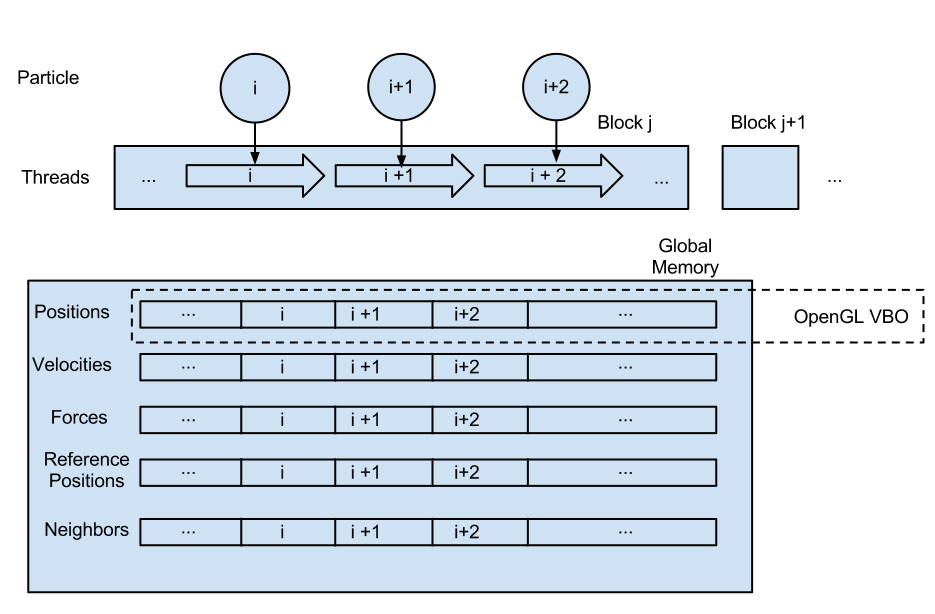
\includegraphics[width = 5in]{Figures/threadDecomp.png}
\caption{Decomposition of the algorithm onto the GPU.}
\label{fig:mapping}
\end{centering}
\end{figure}

There are several points in the algorithm that require global synchronization.  For example, a particle needs to wait for all neighboring particles to apply forces to it before integrating in time.  To handle this, we used several separate CUDA kernels.  This causes more scheduling overhead, but since we are not copying data, this will likely not have a significant performance impact for large simulations.  Figure \ref{fig:kernelDivision} illustrates this division.  Additionally, atomic addition is required to ensure that a particle accounts for forces from all neighboring particles.

\begin{figure}
\begin{centering}
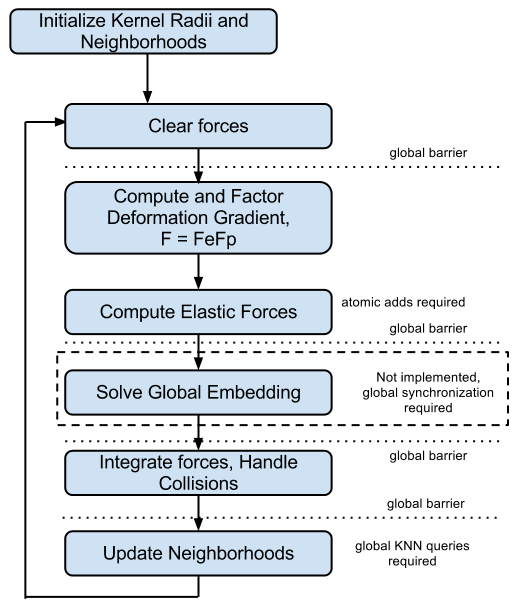
\includegraphics[width = 3in]{Figures/AlgorithmFlowchart.png}
\caption{Overview or required synchronization.}
\label{fig:kernelDivision}
\end{centering}
\end{figure}

\section{Rendering with OpenGL}

????
\begin{figure}
\begin{centering}
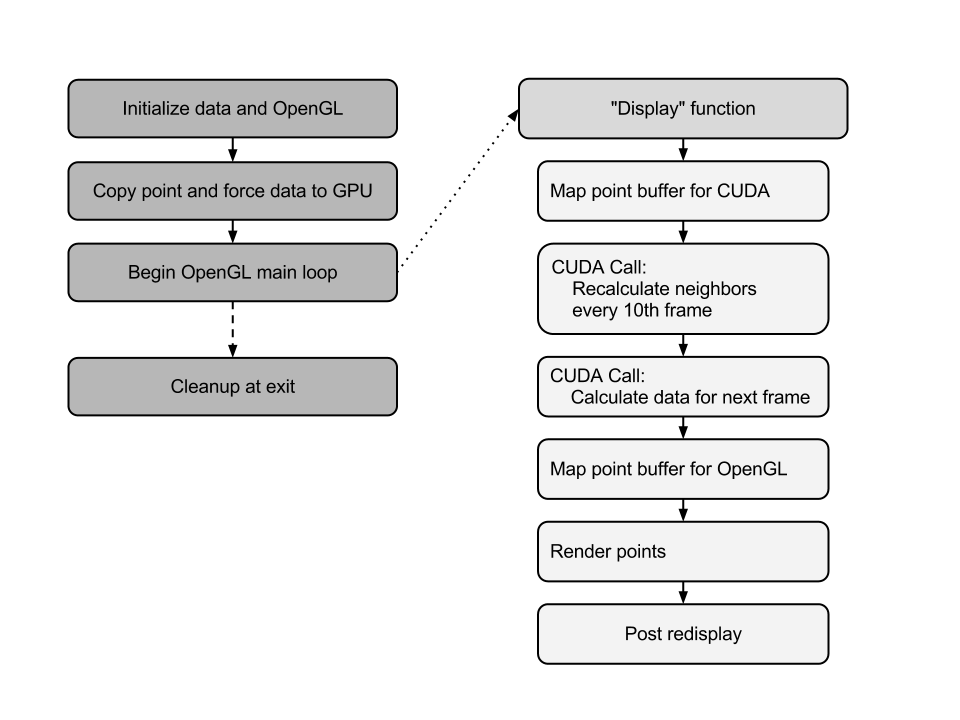
\includegraphics[width = 5in]{Figures/openglFlowchart.png}
\caption{Overview or control flow between OpenGL and CUDA.}
\label{fig:kernelDivision}
\end{centering}
\end{figure}


%\section{Intellectual Challenges}
%
%We expect the biggest challenges to come from solving the sparse matrices.
%These will be large matrices and care will need to be taken to break them up effectively for parallel computation.
%That much is relatively straightforward and similar to previous assignments, but it will be further complicated by the use of sparse matrix methods.
%
%Aside from that, much of the simulation parallelization should simply involve converting loops into threaded CUDA functions, 
%although atomic operations or other synchronization methods may be necessary when calculating interactions between neighboring particles.
%
%Additionally, there may be some challenges in implementing the OpenGL rendering of the simulation.  
%Such difficulties will be due more to unfamiliarity with the process and libraries rather than it being theoretically difficult, 
%since CUDA already has functions that provide the ability to coordinate with OpenGL for rendering purposes.
%
%\begin{CRcatlist}
  %\CRcat{I.3.7}{Computer Graphics}{Three-Dimensional Graphics and Realism}{Animation};
  %\CRcat{I.6.8}{Simulation and Modeling}{Types of Simulation}{Animation}.
%\end{CRcatlist}

%\keywordlist


%----------------------------------------------------------------------------
%----------------------------------------------------------------------------




%\let\ORIGCaption\caption
%\renewcommand{\caption}[1]{\vspace{-0.025in}\ORIGCaption{#1}}

%----------------------------------------------------------------------------
%----------------------------------------------------------------------------


\bibliographystyle{acmsiggraph-awb}
\bibliography{elastoplasticCuda}

\end{document}

